\chapter{Execution of Story Diagrams}

In general, there are two possibilities to execute models: Executing them directly using an interpreter\cite{GHS09} or generating GPL code, which is either compiled or interpreted. Fujaba generates Java (or other code). Here, a story diagram describes the behavior of a single method. Therefore, this method and its containing class must be defined first. Interpreting a story diagrams does not  impose this restriction. 



\section{Interpreting Story Diagrams}

\subsection{Interpreter Architecture}

\begin{figure}[htb]
  \centering
  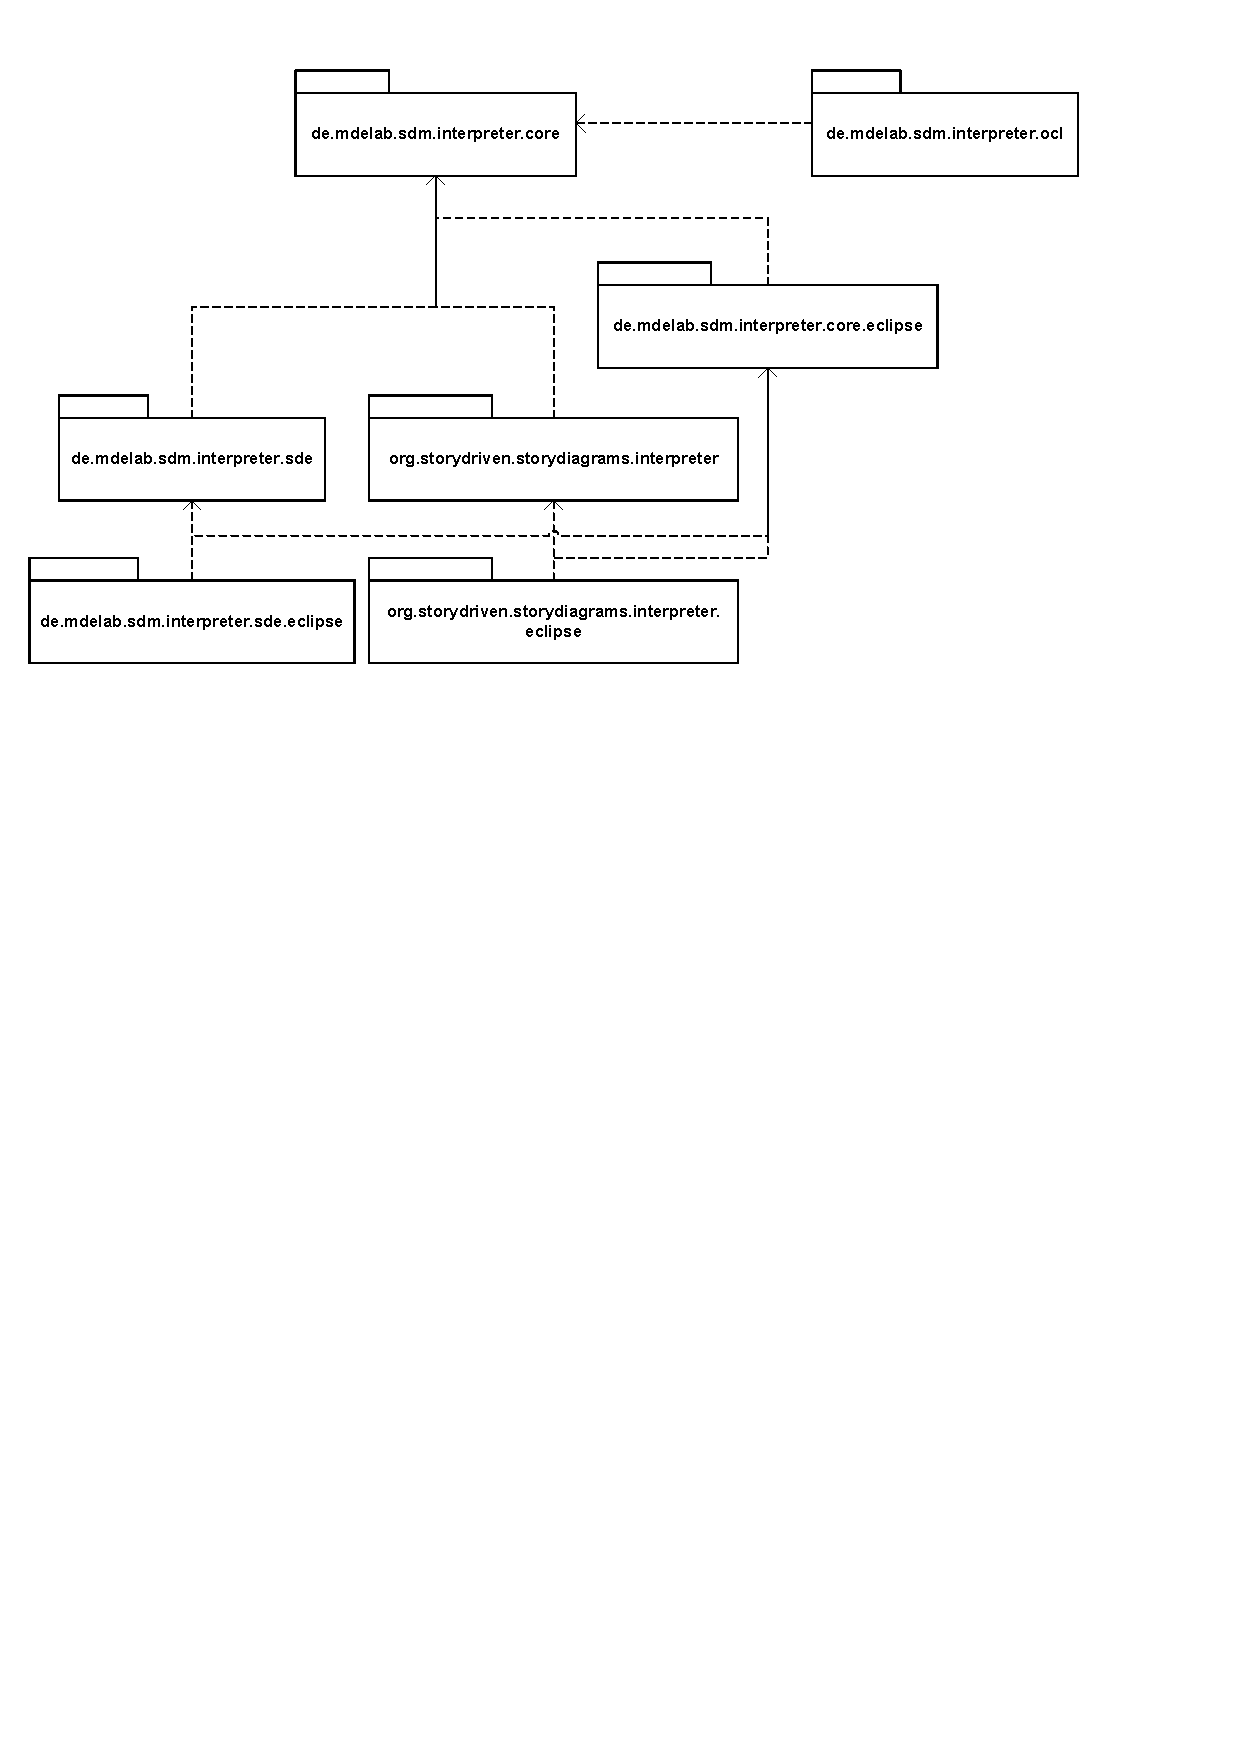
\includegraphics[width=1.0\columnwidth]{./figures/interpreter_packages.pdf}
  \caption{Overview of the packages of the interpreter}
  \label{fig:interpreter_packages}
\end{figure}

Fig.~\ref{fig:interpreter_packages} shows the package structure of the SDM interpreter. The interpreter is divided into a metamodel-independent core (\emph{de.mdelab.sdm.interpreter.core})  and multiple metamodel-dependent extensions (\emph{org.storydriven.modeling.interpreter} and \emph{de.mdelab.sdm.interpreter.sde}). Currently, multiple story diagram metamodels are in use that must all be supported by the interpreter. This separation of metamodel-dependent and independent parts allows for easier maintenance of the interpreter. The classes of the core package define a quite extensive list of generic type parameters (not shown in the subsequent class diagrams), e.g., for activity nodes, classifiers, or features. Subclasses in the metamodel-dependent packages replace these generic types with the concrete types defined in the respective metamodel.

Furthermore, those parts of the interpreter that depend on Eclipse are also separated (\emph{*.eclipse} packages). This allows to use the interpreter in stand-alone applications without Eclipse. In addition, the interpreters for expression languages like OCL are also separated (\emph{de.mdelab.sdm.interpreter.ocl}). The SDM interpreter provides an extension mechanism to add interpreters for other expression languages.

\subsubsection{SDM Interpreter}
\label{sec:sdm_interpreter}

\begin{figure}[htb]
  \centering
  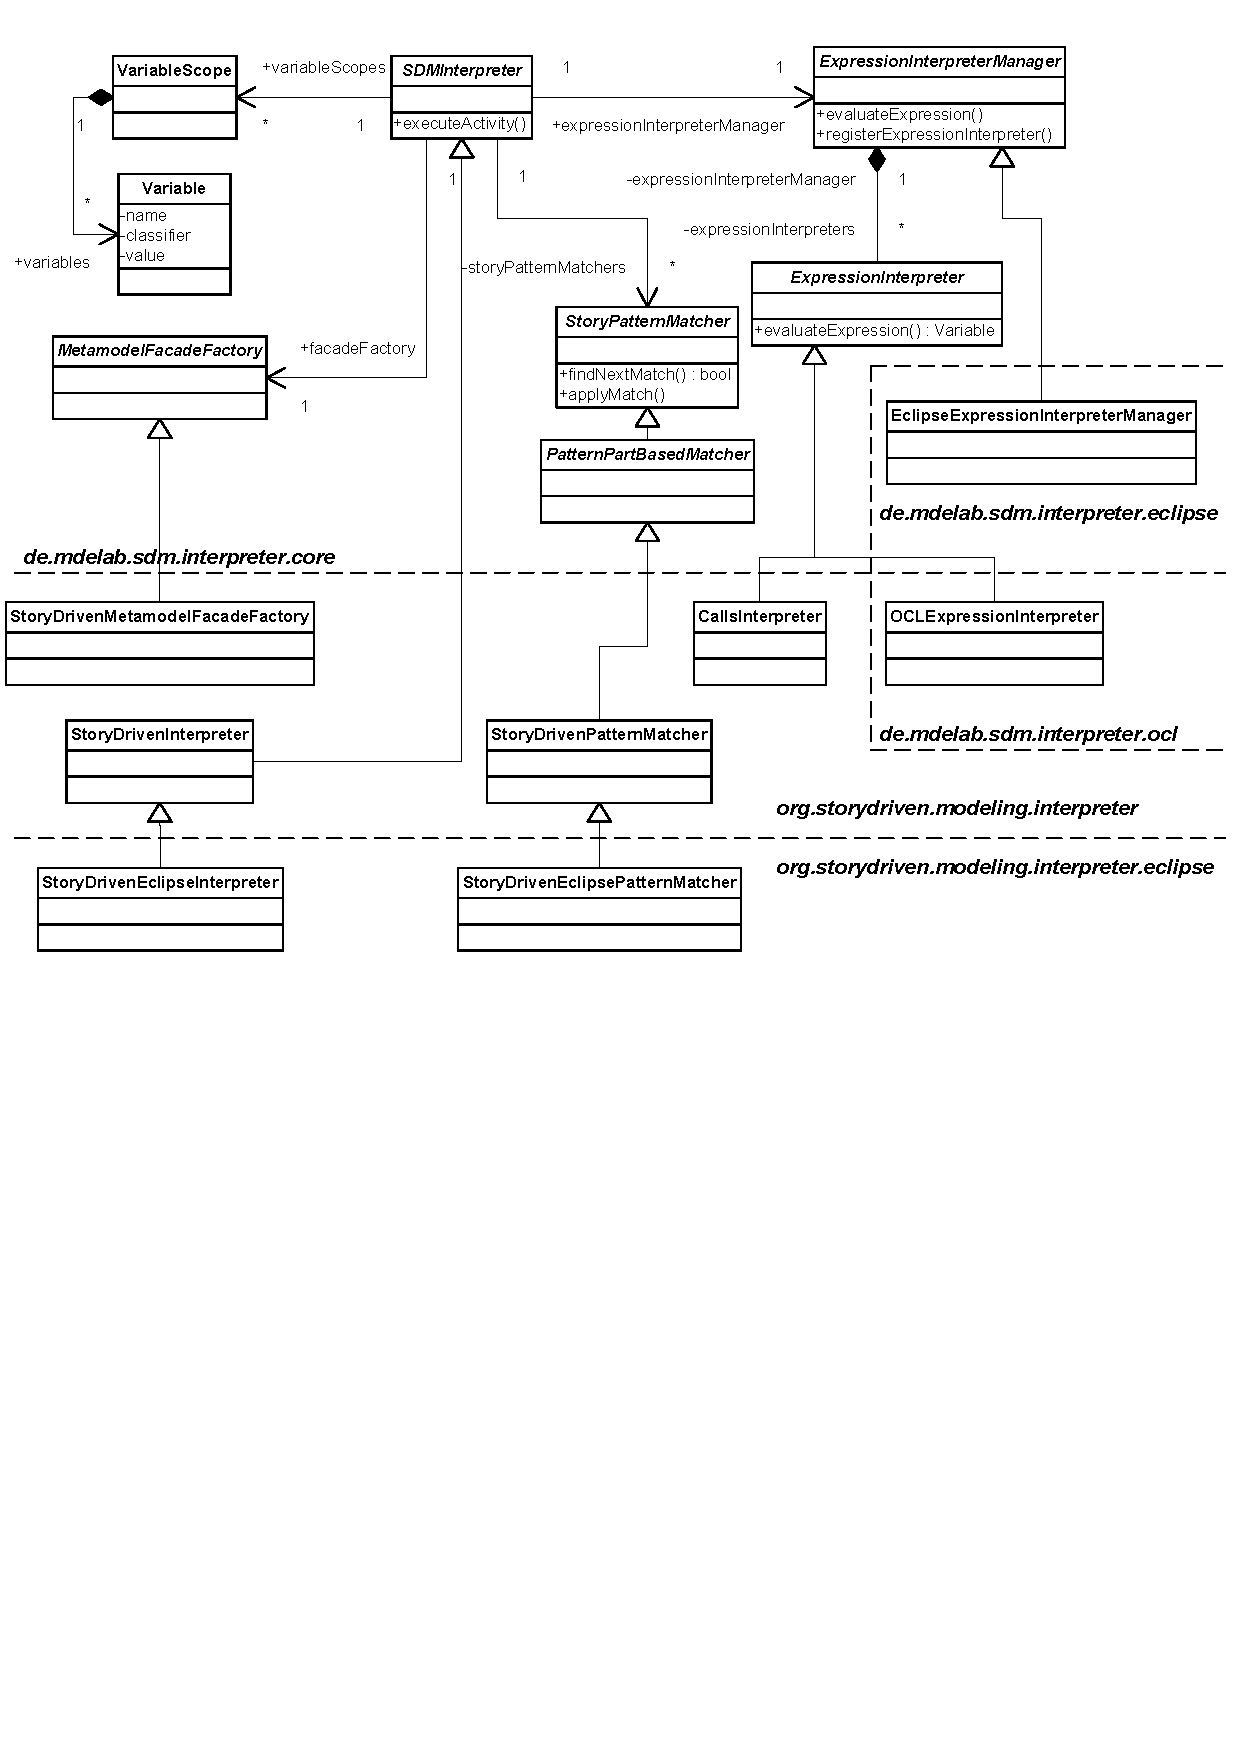
\includegraphics[width=1.0\columnwidth]{./figures/interpreter_core.pdf}
  \caption{Main classes of the interpreter core}
  \label{fig:sdm_interpreter}
\end{figure}

Fig.~\ref{fig:sdm_interpreter} shows the main classes of the interpreter core. \emph{SDMInterpreter} is the abstract superclass of all SDM interpreters. It is responsible for the execution of a whole story diagram. \emph{StoryDrivenInterpreter} and \emph{StoryDrivenEclipseInterpreter} inherit from it to implement metamodel specific functionality. Here, this is mostly limited to defining the concrete types to use in place of the generic types of the superclass and defining constructors with less parameters. The \emph{SDMInterpreter} provides the \emph{executeActivity()} method to execute a story diagram.

\todoall{Is there already a definition of scopes in story diagrams?}

A \emph{VariableScope} is a collection of \emph{Variable}s that are valid in a specific scope. Such a scope can be, e.g., a whole story diagram, a single activity node, or the body of a loop. The \emph{SDMInterpreter} maintains multiple \emph{VariableScope}s for each story diagram element that has an own scope. Currently, there is only one scope for the whole story diagram. A \emph{Variable} is a triple of a name, a classfier, and a value of a variable.

The \emph{ExpressionInterpreterManager} is responsible for managing the interpreters for expression languages and delegating the evaluation of an expression to the appropriate \emph{ExpressionInterpreter}. The \emph{evaluateExpression()} method is provided for that purpose. \emph{ExpressionInterpreter}s have to be registered at the \emph{ExpressionInterpreterManager} via the \emph{registerExpressionInterpreter()} method to be able to evaluate expressions of that language. The \emph{EclipseExpressionInterpreterManager} performs this registration automatically. The plug-in \emph{de.mdelab.sdm.interpreter.eclipse} defines an extension point for \emph{ExpressionInterpreter}s. All interpreters extending this extension point are registered automatically by the \emph{EclipseExpressionInterpreterManager}.

The abstract class \emph{ExpressionInterpreter} only defines the \emph{evaluateExpression()} method that must be implemented by subclasses such as the \emph{OCLExpressionInterpreter} and the \emph{CallsInterpreter}.

At several points in the interpreter, specific properties of story diagram elements have to be accessed, e.g., the name of elements or incoming and outgoing edges of activity nodes. While the interpreter core is metamodel-independent, a facade is required to access these properties. the \emph{MetamodelFacadeFactory} provides access to these facades. More information can be found in Sec.~\ref{sec:metamodel_facades}.

A \emph{StoryPatternMatcher} is responsible for the execution of a single story pattern. This abstract superclass defines the methods \emph{findNextMatch()} to search for the next match of a story pattern and \emph{applyMatch()} to execute the graph transformation on the last match. The class \emph{StoryPatternMatcher} does not implement a particular matching strategy. This is done by \emph{PatternPartBasedPatternMatcher}. This pattern matching strategy is explained in more detail in Sec.~\ref{sec:story_pattern_matcher}. 


\subsubsection{Story Pattern Matcher}
\label{sec:story_pattern_matcher}

\begin{figure}[htb]
  \centering
  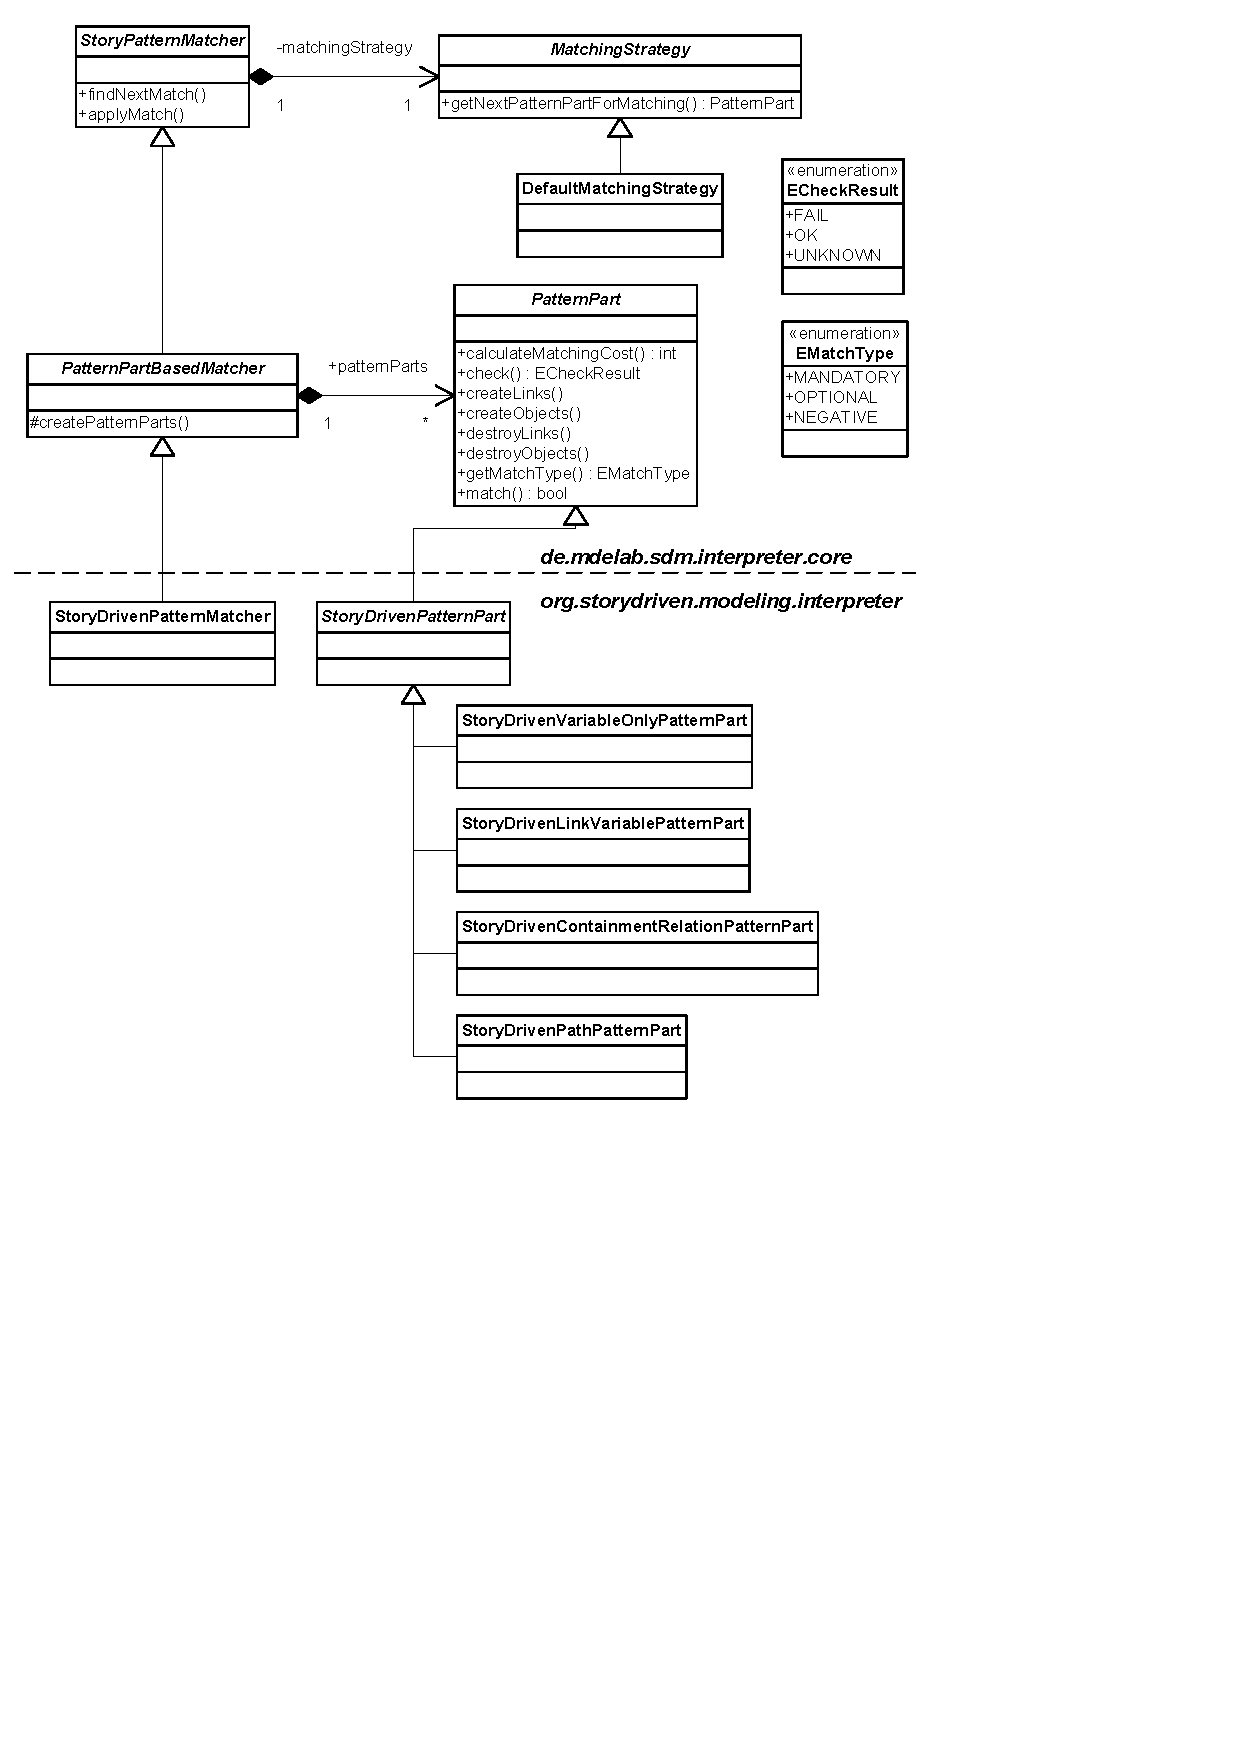
\includegraphics[width=1.0\columnwidth]{./figures/interpreter_storyPatternMatcher.pdf}
  \caption{Main classes of the interpreter core}
  \label{fig:interpreter_storyPatternMatcher}
\end{figure}

Fig.~\ref{fig:interpreter_storyPatternMatcher} shows the classes of the story pattern matcher. Currently, only one specific pattern matching approach is implemented by the class \emph{PatternPartBasedPatternMatcher}. It splits the story pattern into multiple \emph{PatternParts}. What exactly constitutes a \emph{PatternPart} is not specified in the interpreter core. This has to be implemented in the metamodel specific subclasses. Currently, the \emph{StoryDrivenPatternMatcher} enforces the following semantics: A pattern part consists either of a single variable that has no incoming or outgoing links (\emph{VariableOnlyPatternPart}), or of a single link and its adjacent object variables (\emph{StoryDrivenLinkVariablePatternPart}, \emph{StoryDrivenContainmentRelationPatternPart}, and \emph{StoryDrivenPathPatternPart} depending on the kind of link). This implies that a variable can be contained in more than one pattern parts. To implement subpatterns or complex negative application conditions, this semantics has to be modified. But this remains transparent to the basic \emph{PatternPartBasedPatternMatcher}.

\emph{PatternPart} defines several abstract methods: \emph{calculateMatchingCost()} provides an estimate of the cost to match a variable using the link of the pattern part. This estimate can be based, e.g., on the number of elements contained in the link. If it is currently not possible to match this pattern part (e.g., because all variables of the pattern part are still unbound), \emph{-1} is returned. \emph{check()} checks whether the link exists in the instance graph. Of course, the prerequisite is that all variables of the pattern part are already bound to an instance object. If this is not the case, \emph{check()} returns \emph{UNKNOWN}. \emph{createElements()} creates the elements of the pattern part. \emph{destroyLink()} and \emph{destroyObjects()} destroy links and objects. In contrast to the creation of elements, these steps are separated to ensure an orderly deletion of variables in the \emph{VariableScope}. \emph{getMatchType()} returns whether matching the pattern parts is mandatory or optional or the pattern part is a negative application condition. Finally, \emph{match()} implements the pattern matching for this kind of pattern part. For this, at least one variable of the pattern part has to be bound and one unbound. Then, \emph{match()} tries to find matches for all unbound variables. This part of the pattern matching algorithm is highly implementation specific. It is not only different for different metamodels. It also has to be implemented differently for different kinds of links. However, this also allows to exploit certain features of the metamodel to improve performance. For example, \emph{StoryDrivenCointainmentRelationPatternPart} uses EMF's \emph{eContainer()} method to navigate containment links in the opposite direction.

The \emph{MatchingStrategy} determines the order in which pattern parts are matched. The \emph{DefaultMatchingStrategy} matches pattern parts in the order of their matching cost estimates, i.e., \emph{getNextPatternPartForMatching()} returns that pattern part with the lowest cost estimate. 

There are also two additional pattern matching strategies: \emph{DefaultMatchingStrategyWithLog} and \emph{LogReproducingMatchingStrategy}. These are required for \emph{for-each} story nodes. By default for-each story nodes are executed with the fresh-match semantics. Side effects of the story pattern application can influence the pattern matching in subsequent loop iterations, e.g., create new matches or destroy existing matches. They can also influence the pattern matching strategy if they change the number of elements in links. Then, the \emph{DefaultMatchingStrategy} may choose are different order in which pattern parts are matched in the next loop iteration. Because the matching history is discarded during backtracking for the last matched variable, this may cause the pattern matcher to return the same match more than once. Therefore, \emph{DefaultMatchingStrategyWithLog} is used in the first iteration of a for-each story node. It extends \emph{DefaultMatchingStrategy} and logs the order in which pattern parts were matched. \emph{LogReproducingMatchingStrategy} is used in all subsequent iterations of the for-each node and returns the pattern parts to match in the order that the log specifies.

\subsubsection{Metamodel Facades}
\label{sec:metamodel_facades}

\subsubsection{Expression Interpreters}
\label{sec:expression_interpreters}

\subsubsection{Notification Mechanism}
\label{sec:notification_mechanism}

\subsection{Interpreting Story Activities}

The interpretation of the overall story activity starts at the activity's initial node. 




\subsection{Interpreting Story Patterns}


\section{Code Generation for Story Diagrams}
 We don't do it currently. Others have tried that before.\cite{GBD07}